\documentclass[a4paper,12pt]{article}
\usepackage{graphicx}
\usepackage[left=30mm, right=30mm, top=30mm, bottom=30mm]{geometry}
\usepackage{amsmath}
\usepackage{siunitx}
\usepackage{fancyhdr}
\usepackage{url}
\pagestyle{fancy}
%-------------------------------------------------------------------------------
\lhead{\textbf{Spring 2019}}
\rhead{\textbf{CE394M Advanced Analysis in Geotechnical Engineering}}
\cfoot{\thepage}
%-------------------------------------------------------------------------------

\begin{document}
\begin{centering}
	\textbf{
		Assignment 9: Cam-Clay\\
		Assigned: 29th April 2019\\
		Due: 10th May 2019\\
	}
\end{centering}

\vspace{1em}
\section{Simple shear}

\begin{enumerate}
	
	\item Kaolin is reconstituted to a slurry and is then permitted to re-consolidate one-dimensionally. It eventually reaches a vertical effective stress of 100 kPa in a Simple Shear Apparatus:
	\begin{enumerate}
		\item Estimate its water content
		\item Predict its undrained shear strength
		\item It is then permitted to drain while it continues shearing; predict its drained shear strength.
		\item What volumetric change will the sample eventually suffer during its drained shearing? How would this estimate be changed if a pre-consolidation stress of 1000 kPa had first been imposed during the initial setting-up.
	\end{enumerate}

	\item London Clay is normally consolidated to 1000 kPa and then permitted to swell back into equilibrium (with zero pore pressure) under a normal stress of 50 kPa
	\begin{enumerate}
		\item Predict both drained and undrained shear strengths using SSA Cam Clay.
		\item Estimate the pore water pressure consistent with your estimate of the undrained shear strength. Comment on the magnitude in relation to the probable behavior of heavily over-consolidated London Clay exposed in an excavation.
	\end{enumerate}
\end{enumerate}

\section{Triaxial tests}
\begin{enumerate}
	\item Establish expression for TX compression Cam Clay parameter $M$ as a function of $\phi_{crit}$. Assume that the test eventually come to mobilize $\phi_crit$ in the vertical plane. Hint: Use earth pressure co-efficient to relate different component of stresses. 
	
	\item A saturated clay is characterized by these Cam-Clay parameters: $M = 0.87$, $\lambda = 0.091$, $\kappa = 0.035$ and $\Gamma = 2.072$ at $p^\prime = 1 kPa$. 
	Consider two different soil specimens consolidated to the same $p_c^\prime = 100 kPa$. Specimen A is isotropically consolidated to $p_c^\prime = 100 kPa$, while Specimen B is anisotropically consolidated to $p_c^\prime = 100 kPa$ with $K_c = \sigma_{1c}^\prime / \sigma_{3c}^\prime = 2.0$. 
	\begin{enumerate}
		\item Sketch the initial states, paths and yield surfaces for each specimen in $q-p^\prime$ and $v - \ln p^\prime$ space. 
		\item Use the OCC and MCC models to predict the undrained shear strength fro the two speciments. Compare your results.
		\item Use the OCC and MCC models to predict the drained $q_f$ at failure.
	\end{enumerate}

	\item Weald clay is reconstituted as a saturated slurry and isotropically consolidated to $p^\prime = 100kPa$, before being allowed to swell back to 70kPa.
	\begin{enumerate}
		\item What will be its water content?
		\item It is then to be subjected to undrained triaxial compression. At what deviatoric stress $q$ might the sample yield? Estimate the axial strain at yield (assuming effective Poisson's ratio of 0.15).
		\item If $q$ is allowed to increase a further 10\% as the undrained test progresses, search for a consistent value of the mean effective stress $p^\prime$ at that stage.
		\item What ultimate undrained strength $q_u$ should be recorded?
		\item What volumetric strain should occur if the sample were finally allowed to drain while
		shearing continued, and what would be the ultimate strength?
	\end{enumerate}

\end{enumerate}
\begin{figure}[!h]
	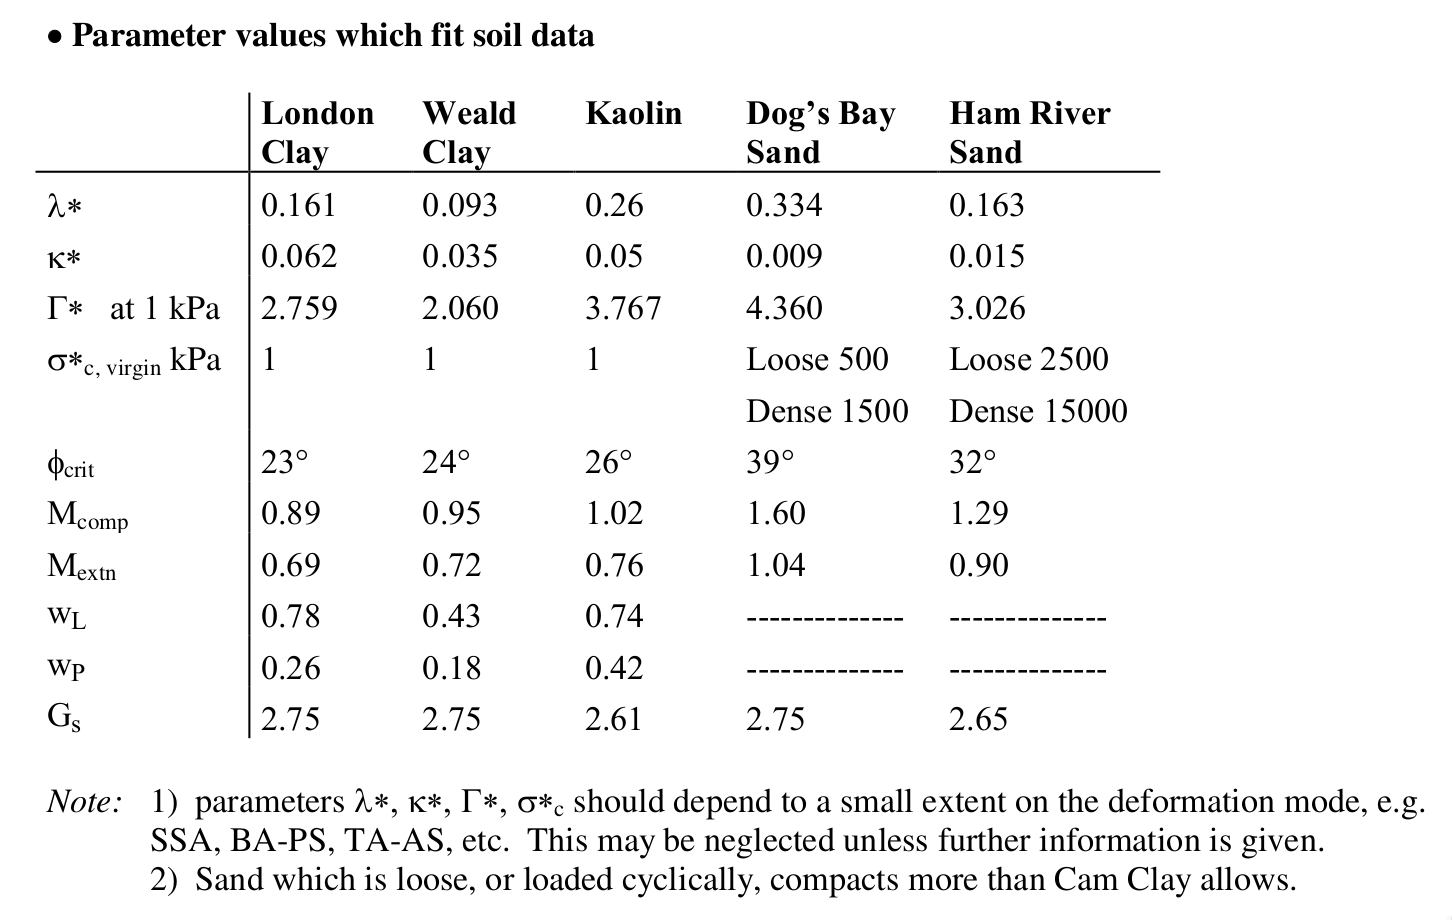
\includegraphics[width=\textwidth]{figs/soil-data-sheet.png}
\end{figure}
\end{document}

